\documentclass[12pt]{article}
\usepackage{graphicx}
\usepackage{hyperref}
\usepackage{float}
\usepackage{graphicx}
\usepackage{caption}
\usepackage{subcaption}

\begin{document}

\title{\textbf{Census Income Classification}}
\author{
    Shubham Pandya\\
    Yishtavi Gedipudi\\
    Atharva Gosavi\\
    Hritik Puri \\
    Raghavi Dube\\
    \\\\
    \texttt{
    pandya.shu@northeastern.edu\\
    gedipudi.y@northeastern.edu\\
    gosavi.at@northeastern.edu\\
    puri.hr@northeastern.edu\\
    dube.ra@northeastern.edu\\}
}
\date{Submission Date: \today}
\maketitle
\newpage

\begin{abstract}
This project analyzes the U.S. Census data from 1994 to predict income levels exceeding \$50,000 using statistical learning techniques. We employ logistic regression, Gaussian Naive Bayes, and Support Vector Machine models to explore which socio-economic factors most significantly impact income levels. Initial data exploration, preprocessing, and extensive exploratory data analysis are conducted to prepare the dataset for modeling. The report details each model's implementation, evaluates their performance, and discusses their suitability based on their inherent trade-offs and predictive accuracy.
\end{abstract}


\newpage

\tableofcontents
\newpage

\section{Introduction}
The U.S. Census Income dataset, commonly referred to as the Adult dataset, is extracted from the 1994 Census database and is a critical resource in the predictive modeling community. It comprises a diverse range of demographic and employment-related variables from approximately 299,285 instances spread across multiple states. This extensive dataset not only encapsulates the complex socio-economic landscape of mid-90s America but also serves as a foundational tool for examining the factors that influence income levels.

The dataset’s primary objective is to predict whether individuals earn above or below \$50,000 annually based on a rich set of features such as age, education, occupation, and hours worked per week, among others. These attributes reflect a broad spectrum of the labor market and demographic distinctions, providing a nuanced understanding of income disparities.

In addition to its primary use in income prediction, the dataset supports a wide range of social science research, offering insights into labor dynamics, economic inequality, and the distribution of wealth across different demographic groups. The data's categorical and continuous nature allows for deep dives into machine learning and statistical analysis, making it an invaluable resource for both academic and practical applications in policy making and economics.

Moreover, the dataset highlights the instance weight, which indicates the number of people each record represents in the population due to stratified sampling methods employed during data collection. This aspect is crucial for accurate analysis and representation in studies aimed at understanding population-wide trends.

Overall, the U.S. Census Income dataset not only provides a snapshot of the economic conditions of the United States in the mid-1990s but also continues to offer a robust framework for exploring the implications of various socio-economic factors on income through the lens of statistical learning methods.

\begin{figure}[H]
    \centering
    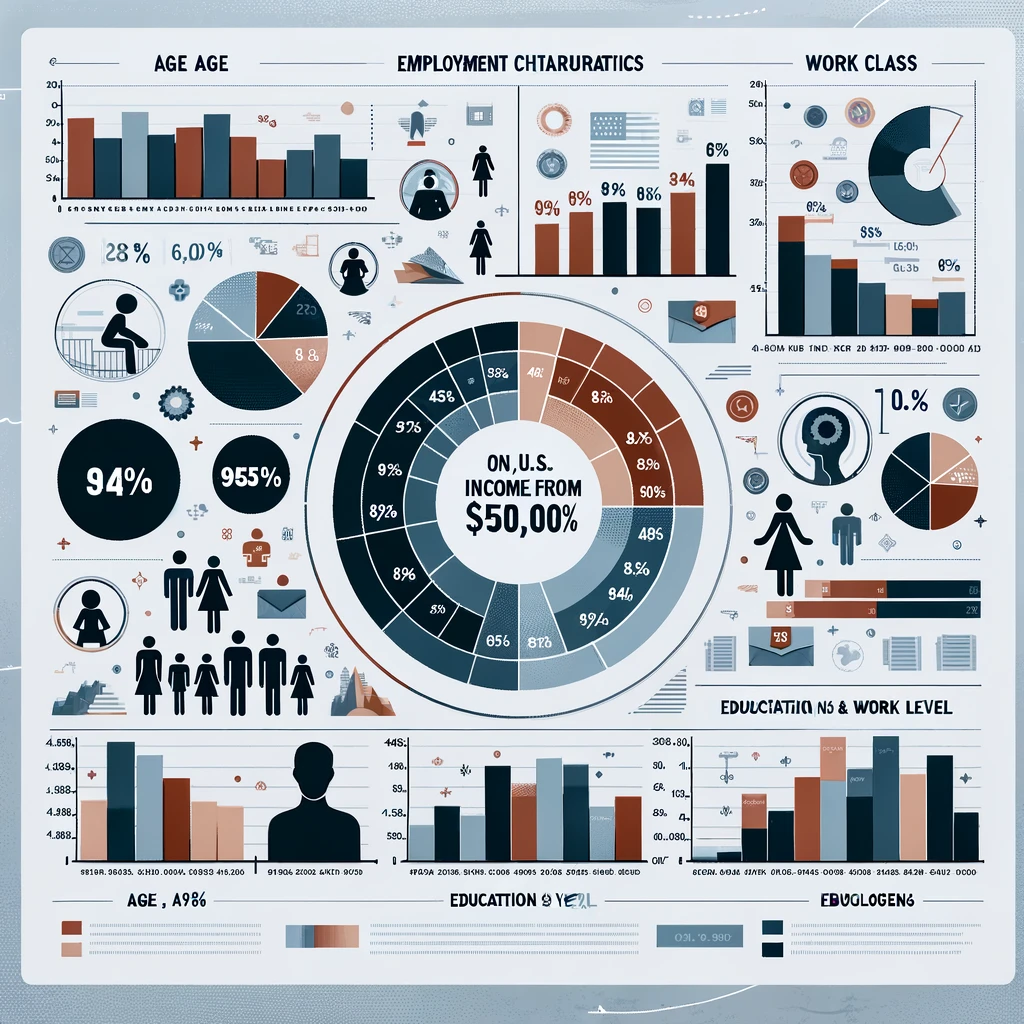
\includegraphics[width=0.8\textwidth]{images/introduction.png}
    \caption{Infographic of Demographic and Employment Characteristics}
\end{figure}
 


\section{Data Description}
The dataset comprises 32,561 entries and includes 15 attributes, detailing demographic and employment-related information crucial for modeling income levels. Here are some insights derived from the visualized data:

\begin{itemize}
    \item Work Class shows a predominant number of individuals employed in the private sector.
    \item Education levels are diverse, with a significant number having a high school education or some college experience.
    \item Marital Status and Occupation distributions underscore varied social and professional dynamics.
    \item Relationship status distribution hints at family structures which could influence economic stability.
    \item Race and Sex distributions reflect demographic diversity, crucial for understanding economic disparities.
\end{itemize}
 \begin{figure}[H]
    \centering
    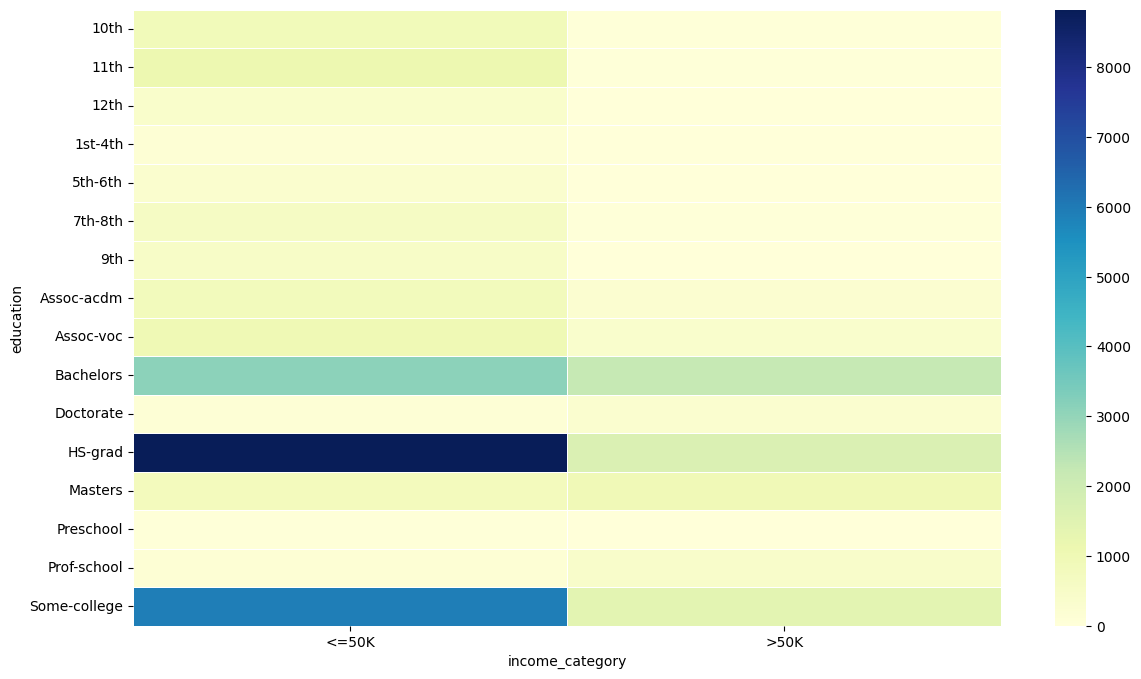
\includegraphics[width=0.8\textwidth]{images/data_description_1.png}
    \caption{Description}
\end{figure}
\begin{figure}[H]
    \centering
    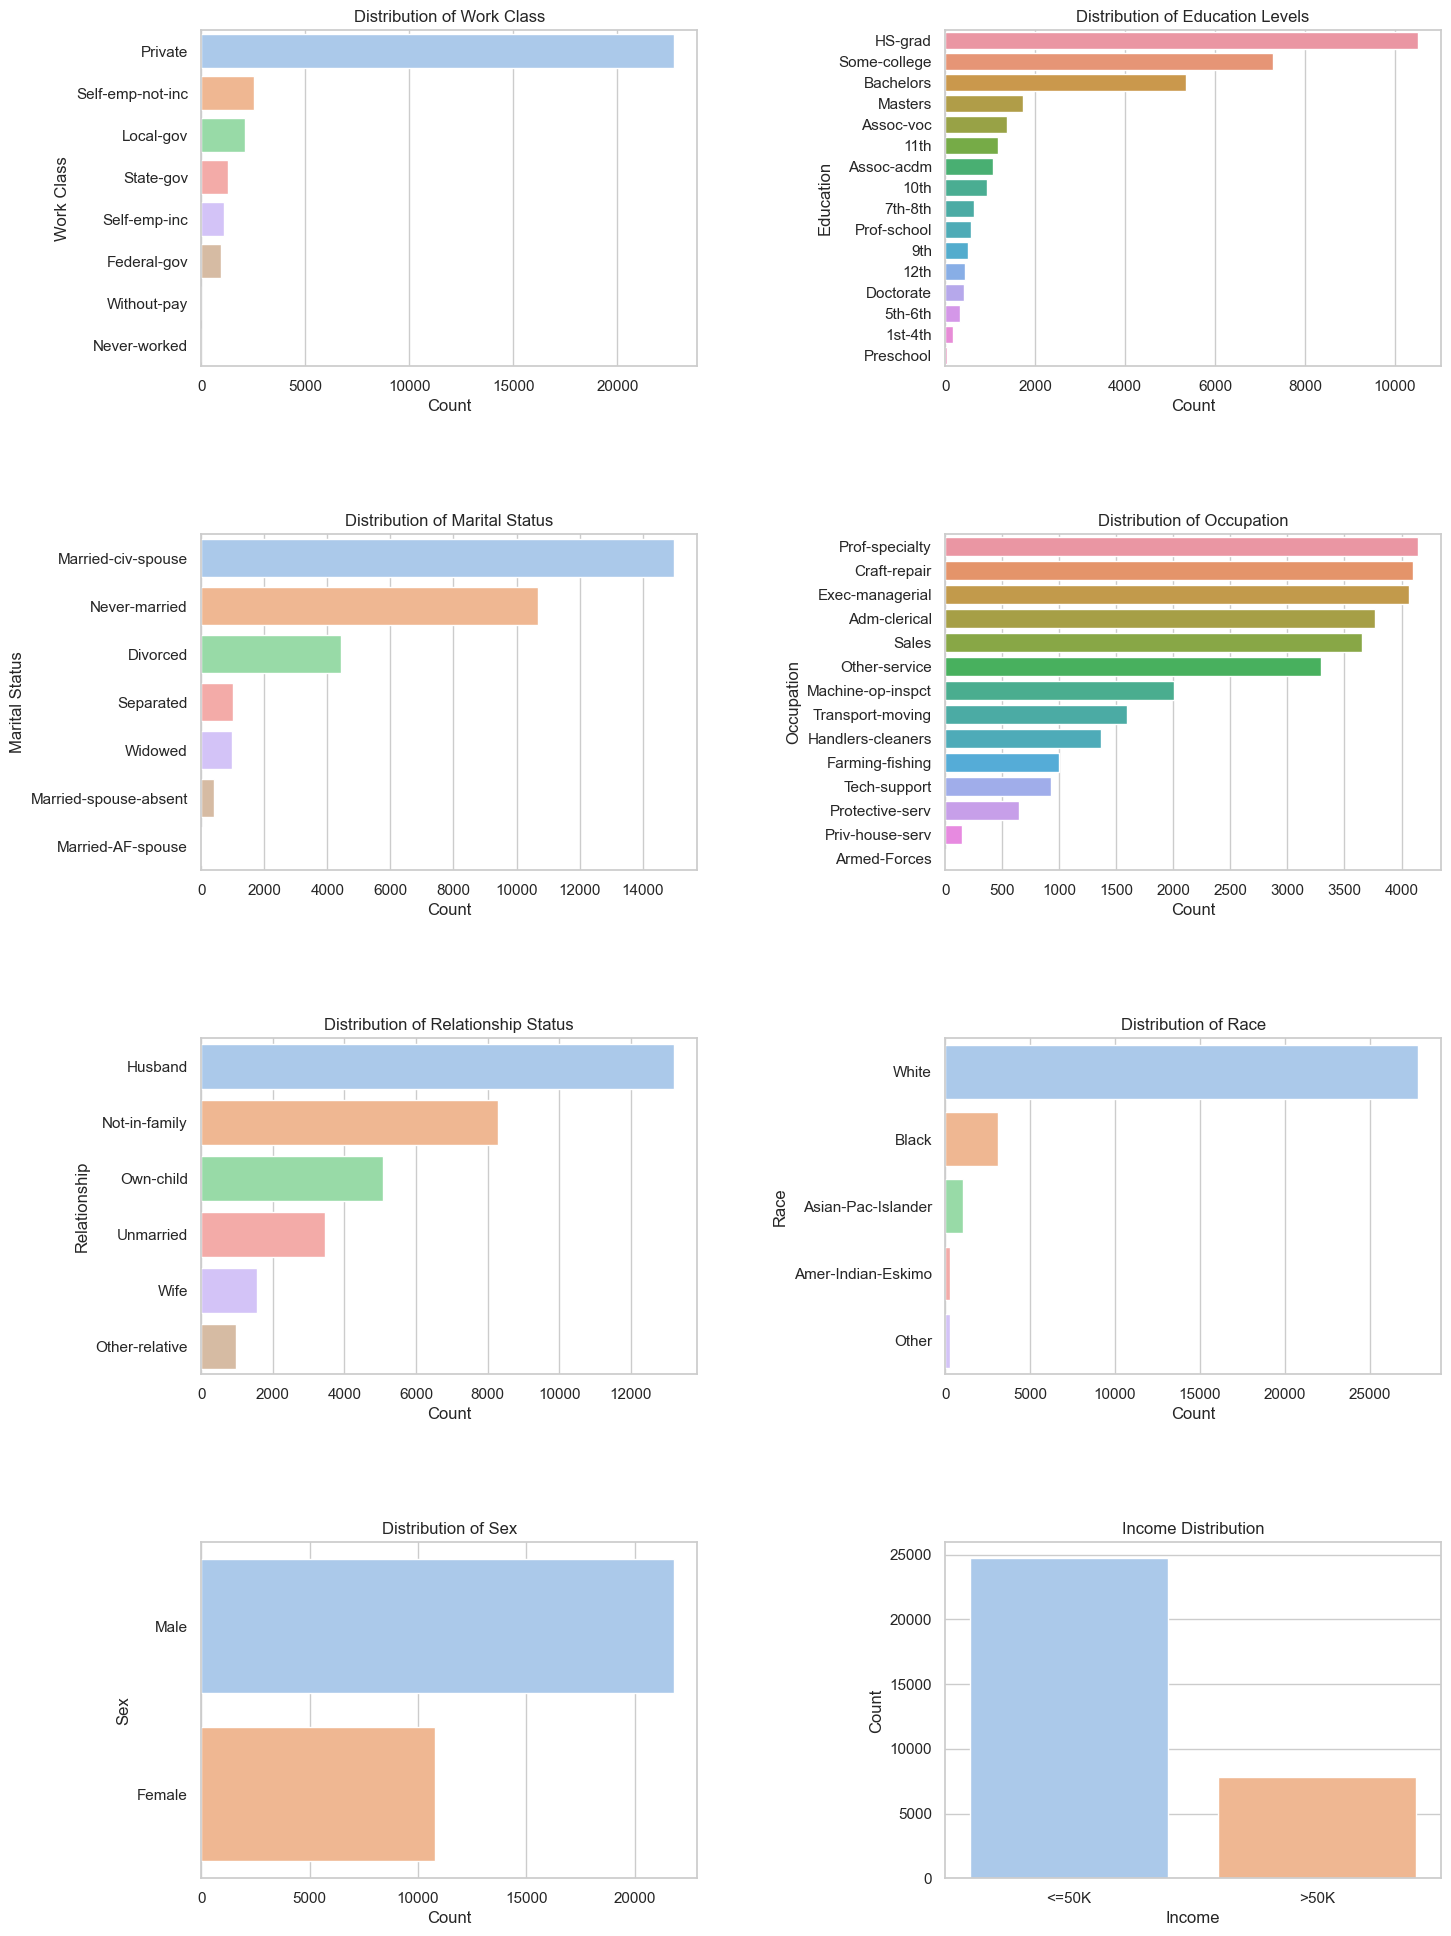
\includegraphics[width=0.8\textwidth]{images/data_description_2.png}
    \caption{Description}
\end{figure}

\section{Data Cleaning and Pre-processing}
The dataset underwent several preprocessing steps to ensure data quality and consistency:
\begin{itemize}
    \item Removal of trailing periods in the income category to unify the format across the training and test datasets.
    \item Stripping spaces from categorical variables, improving the consistency of data entries.
    \item Dropping unnecessary columns like 'education' which duplicated 'education\_num'.
    \item Removal of duplicate records to ensure unique entries for analysis.
    \item Standardization of the 'income' field by removing periods and adjusting spaces.
\end{itemize}

\section{Exploratory Data Analysis}
This section provides a comprehensive view of the dataset's key features, illustrating the distribution and relationships within the data. The visualizations are organized to present a clear comparative analysis across different demographic and economic variables.
\begin{figure}[H]
    \centering
    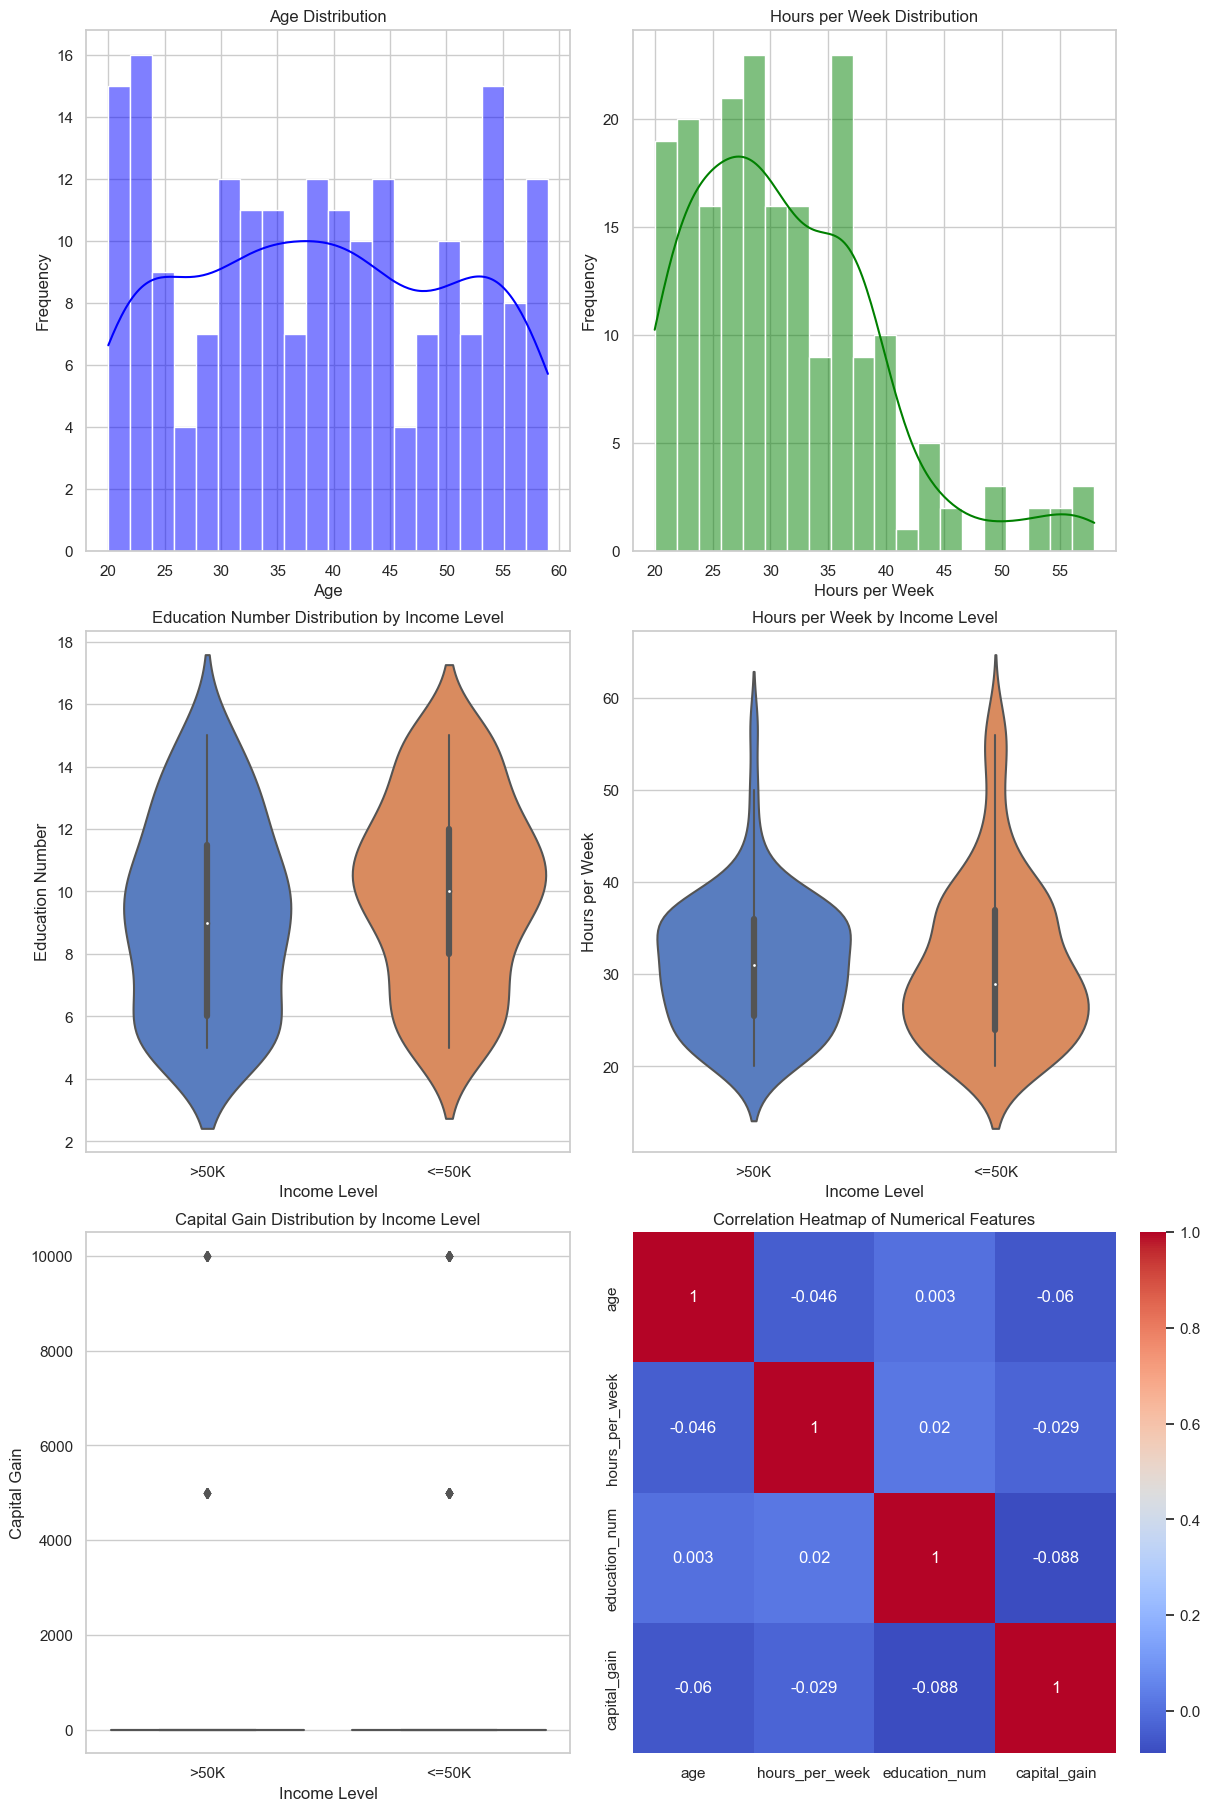
\includegraphics[width=\textwidth]{images/eda.png}
    \caption{Comprehensive Data Analysis across multiple demographics and economic variables.}
\end{figure}
\subsection{Analysis}
Detailed analysis of the visualizations revealed several key insights:
\begin{itemize}
    \item Age and weekly working hours show varied patterns across different income levels, suggesting that both factors are influential in income disparity.
    \item Higher education levels and significant capital gains are more prevalent among those with incomes above \$50K, highlighting the impact of education and investment on income.
    \item The correlation heatmap provides insights into the relationships between numerical features, showing moderate correlations that could influence model building.
\end{itemize}

\section{Methodology}
This section describes the statistical models and machine learning techniques used in the analysis, focusing on their theoretical foundations, advantages, and disadvantages.

\subsection{Logistic Regression}
Logistic Regression, often referred to as the logit model, is a statistical model used for classification and predictive analytics. It estimates the probability of an event occurring based on a set of independent variables, with the outcome constrained between 0 and 1 (e.g., probability of an individual earning above \$50,000).

\textbf{Advantages:}
\begin{itemize}
    \item Easy to implement, interpret, and very efficient to train.
    \item Does not assume distributions of classes in feature space.
\end{itemize}

\textbf{Disadvantages:}
\begin{itemize}
    \item Not suitable when the number of observations is less than the number of features; may lead to overfitting.
    \item Only constructs linear boundaries.
\end{itemize}

\subsection{Naïve Bayes}
The Naive Bayes classifier is based on Bayes' Theorem and is used for solving classification problems. It is a fundamental yet powerful algorithm that operates under the assumption that each feature makes an independent and equal contribution to the outcome.

\textbf{Advantages:}
\begin{itemize}
    \item Fast and efficient, suitable for large datasets and multi-class prediction problems.
\end{itemize}

\textbf{Disadvantages:}
\begin{itemize}
    \item Assumes independence among predictors, which is rarely the case in real life.
    \item Probability outputs are not always reliable.
\end{itemize}

\subsection{Support Vector Machine (SVM)}
Support Vector Machine or SVM is a popular algorithm used for both classification and regression. However, it is primarily used for classification problems. SVM constructs a hyperplane or set of hyperplanes in a high-dimensional space to separate different classes.

\textbf{Advantages:}
\begin{itemize}
    \item Provides good generalization capabilities, preventing over-fitting through the L2 norm.
    \item Can handle non-linear data using Kernel trick.
\end{itemize}

\textbf{Disadvantages:}
\begin{itemize}
    \item Computationally intensive, particularly with large datasets.
    \item Selection of a suitable kernel function can be complex and critical for performance.
\end{itemize}

\textit{[Following this theoretical framework, the subsequent sections will provide a detailed implementation and evaluation of each model.]}

\section{Logistic Regression Model Implementation}

Logistic regression is a supervised learning algorithm designed for classification problems. It predicts the probability that a new example belongs to a particular class by mapping a function from the input features to the target classes. The goal of logistic regression is to understand categorization and why linear regression is unsuitable for categorical outputs. 

In our project, we used logistic regression for a binary classification problem, identifying whether an event occurs (1) or not (0). We started by applying the logistic function, also known as the sigmoid function, defined as:
\[ h(t) = \frac{1}{1 + e^{-t}} \]
This function constrains the output to a probability between 0 and 1.

The cost function, or log-loss, for logistic regression is defined as:
\[ \text{Cost}(h(t), y) = \begin{cases} 
- \log(h(t)) & \text{if } y = 1 \\
- \log(1 - h(t)) & \text{if } y = 0 
\end{cases} \]
This configuration penalizes incorrect class predictions by the model, with the penalty increasing as the prediction deviates from the actual class.

To optimize our model, we used gradient descent to minimize the cost function. The approach involves:
1. Computing the derivative of the cost function to determine the direction of the steepest descent.
2. Adjusting the parameters proportionally to the negative of the gradient multiplied by the learning rate to find the global minimum of the cost function.


\subsection{Data Encoding and Preparation}
We confirmed that all but one of our columns are numeric after preprocessing, with the income variable being the sole non-numeric column used as the target for our predictions. One-hot encoding transformed categorical variables into a format suitable for modeling, resulting in 92 feature columns.

\subsection{Model Training}
Our logistic regression model was trained using a learning rate of 0.01 over 500 iterations with L2 regularization (lambda=0.1). The training process optimized the model weights to minimize the cost function, representing the prediction error.

\subsection{Performance Metrics}
The model's learning curve, a plot of the cost function over iterations, displayed a descending trend, indicating effective learning (Figure \ref{fig:learning_curve}). Performance metrics, plotted over iterations, revealed an increase in accuracy and precision, and a decrease in recall, suggesting that our model progressively learned to correctly predict a larger portion of the income classifications (Figure \ref{fig:metrics}).

\subsection{Confusion Matrix}
The confusion matrix provided a detailed breakdown of the model's predictive performance on the test data, highlighting the true positives, true negatives, false positives, and false negatives (Figure \ref{fig:confusion_matrix}).

\subsection{Receiver Operating Characteristic (ROC)}
We also plotted the ROC curve, which shows the trade-off between the true positive rate and false positive rate at various threshold settings. The area under the curve (AUC) was 0.88, indicating a high level of model discriminative ability (Figure \ref{fig:roc_curve}).

\subsection{Classification Report}
The classification report shows the precision, recall, and F1-score for both classes along with the support, which is the number of true instances for each label:

\begin{table}[H]
\centering
\begin{tabular}{|l|c|c|c|c|}
\hline
\textbf{Class} & \textbf{Precision} & \textbf{Recall} & \textbf{F1-Score} & \textbf{Support} \\ \hline
<=50K & 0.81 & 0.76 & 0.78 & 4934 \\ \hline
>50K & 0.77 & 0.83 & 0.80 & 4945 \\ \hline
\multicolumn{1}{|r|}{\textit{Accuracy}} & \multicolumn{4}{c|}{0.79} \\ \hline
\multicolumn{1}{|r|}{\textit{Macro Avg}} & 0.79 & 0.79 & 0.79 & 9879 \\ \hline
\multicolumn{1}{|r|}{\textit{Weighted Avg}} & 0.79 & 0.79 & 0.79 & 9879 \\ \hline
\end{tabular}
\caption{Classification report for the logistic regression model.}
\label{tab:classification_report}
\end{table}


The following figures elucidate the detailed analysis and results of the logistic regression model applied to the U.S. Census Income dataset.

\begin{figure}[H]
\centering
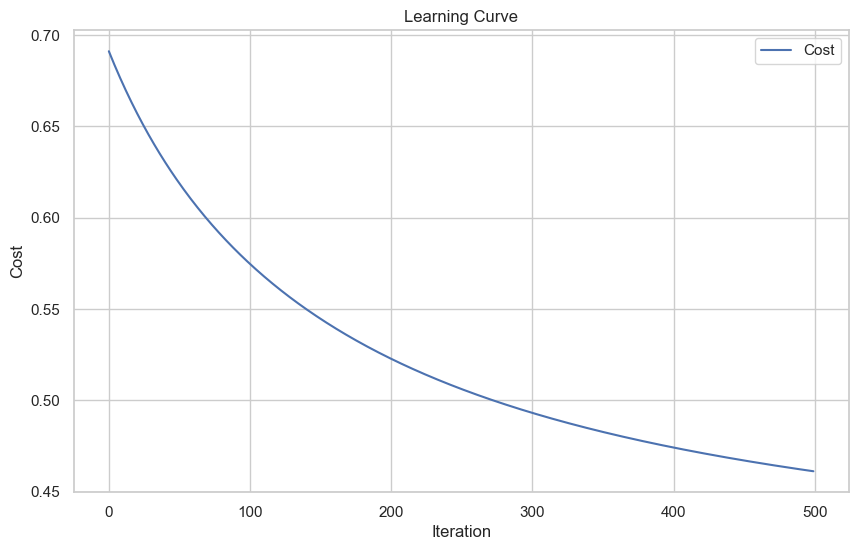
\includegraphics[width=0.8\textwidth]{images/Linear_Learning_curve.png}
\caption{Learning curve of the logistic regression model.}
\label{fig:learning_curve}
\end{figure}

\begin{figure}[H]
\centering
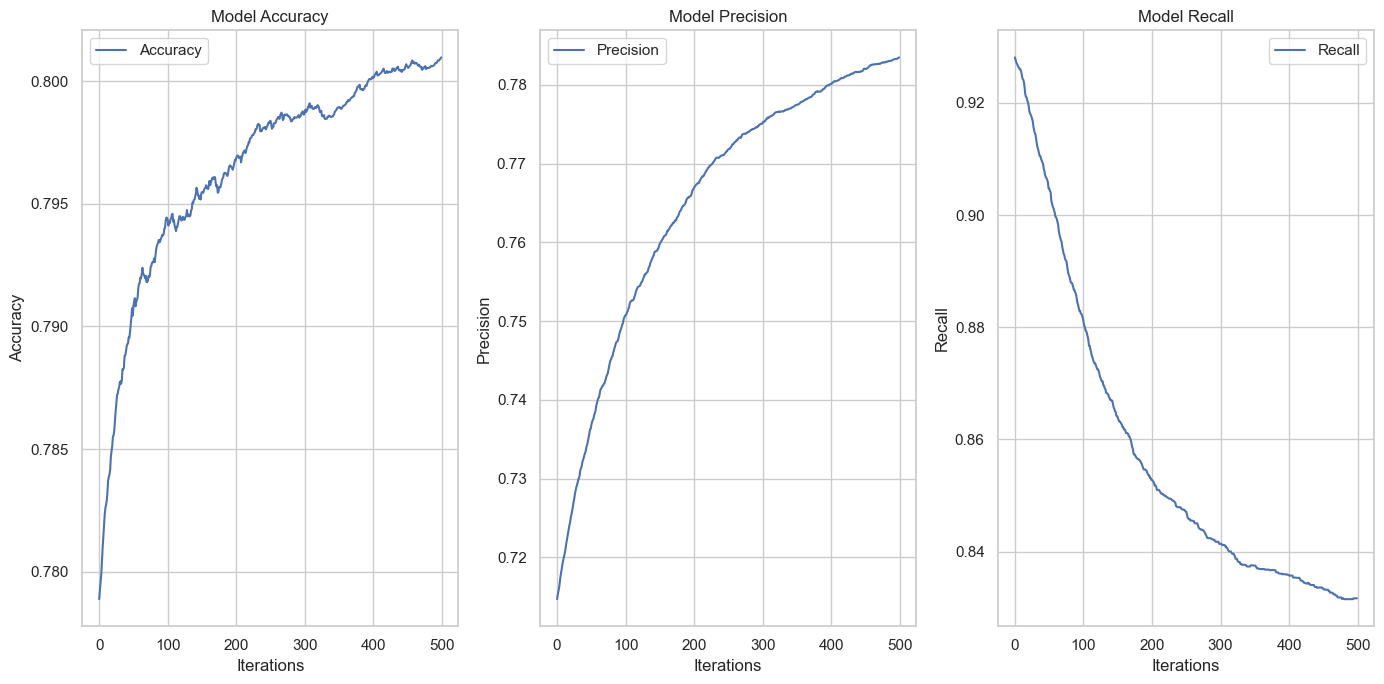
\includegraphics[width=0.8\textwidth]{images/Linear_Learning_rest.png}
\caption{Accuracy, Precision, and Recall over iterations.}
\label{fig:metrics}
\end{figure}

\begin{figure}[H]
\centering
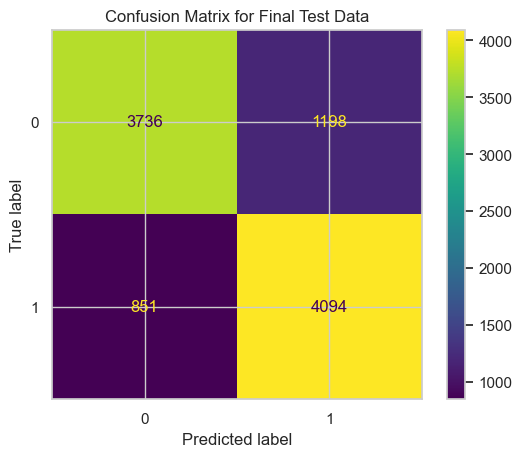
\includegraphics[width=0.8\textwidth]{images/logistic_confusion_1.png}
\caption{Confusion Matrix for Final Test Data.}
\label{fig:confusion_matrix}
\end{figure}

\begin{figure}[H]
\centering
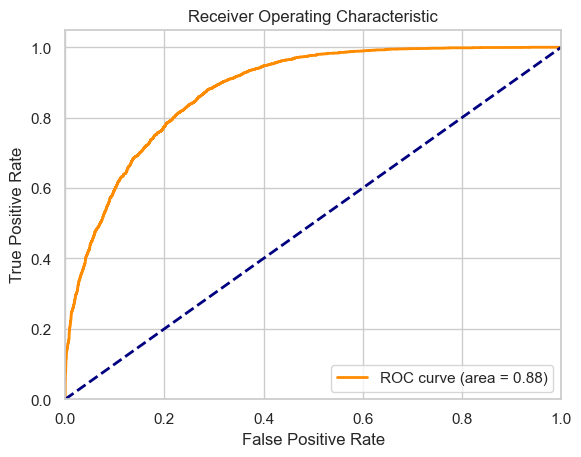
\includegraphics[width=0.8\textwidth]{images/logistic_roc.png}
\caption{Receiver Operating Characteristic curve.}
\label{fig:roc_curve}
\end{figure}

\newpage
\section{Gaussian Naive Bayes Model Implementation}
Naive Bayes Classification, based on Bayes' Theorem, is a generative technique. It assumes that all features contribute independently to the probability of each class, making it particularly suited for cases where features are conditionally independent given the class.

For our continuous and binary categorical target data, we applied the Gaussian Naive Bayes approach:
\[ P(X_k | Y = j) \sim N(\mu, \sigma^2) \]
\[ P(X_k | Y = j) = \frac{1}{\sqrt{2\pi} \sigma} e^{-\frac{(x-\mu)^2}{2\sigma^2}} \]

Initially, we separated our training data by class to calculate prior probabilities:
\[ P(Y = 0) = \frac{\text{Count of `0' labels}}{\text{Total data points}} \]
\[ P(Y = 1) = \frac{\text{Count of `1' labels}}{\text{Total data points}} \]

Using these priors and the likelihoods from the Gaussian distribution, we computed class probabilities for new data points. To address the limitation of zero likelihoods, we implemented Laplace smoothing, adjusting zero probabilities to a small constant value to ensure that no class probability becomes zero.


\begin{figure}[H]
\centering

\caption{Model training output for Gaussian Naive Bayes.}
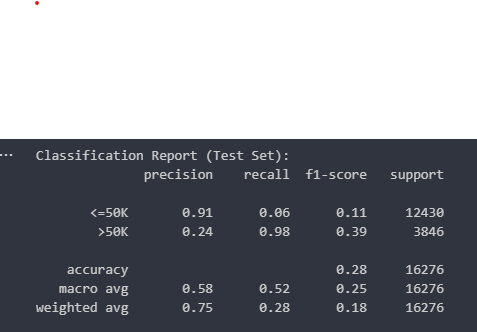
\includegraphics[width=\textwidth]{images/gnb_output.png}
\end{figure}

\begin{figure}[H]
\centering
\caption{Confusion Matrix for the Training Set.}
\end{figure}
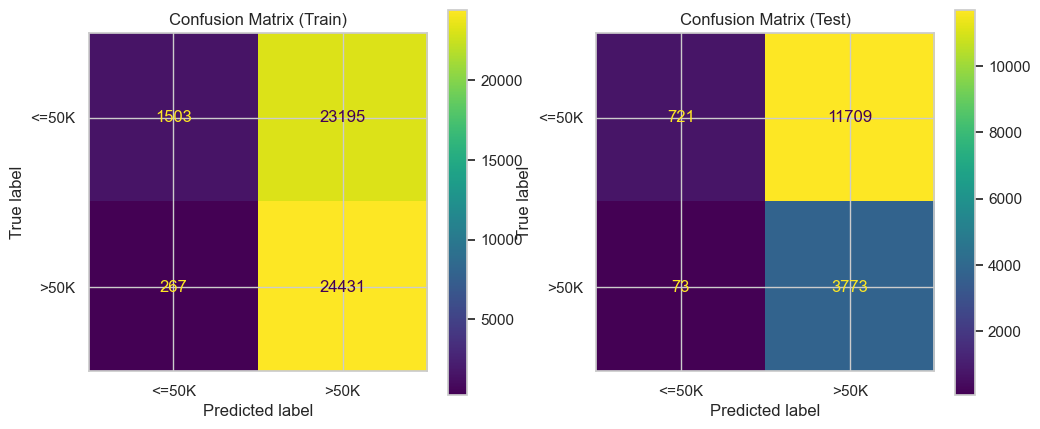
\includegraphics[width=\textwidth]{images/gnb_confusion.png}

\begin{figure}[H]
    \centering
    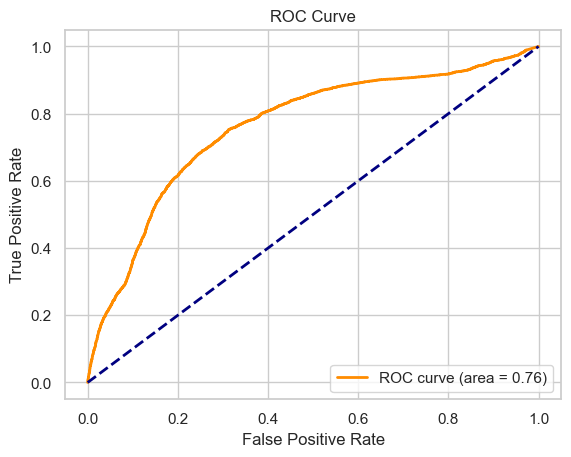
\includegraphics[width=\textwidth]{images/gnb_roc.png}
    \caption{ROC Curve for Gaussian Naive Bayes Model.}
\end{figure}

\begin{figure}[H]
\centering
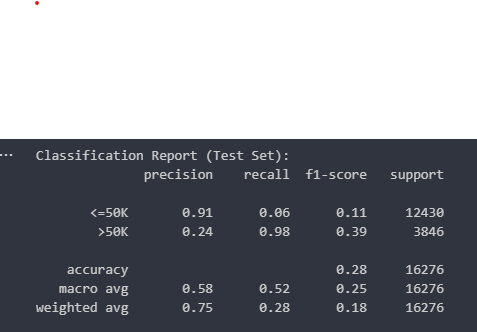
\includegraphics[width=\textwidth]{images/gnb_output.png}
\caption{Classification report for the Gaussian Naive Bayes model.}
\end{figure}
\section{Support Vector Machine (SVM) Implementation}

The SVM algorithm constructs an optimal hyperplane in an n-dimensional space that categorizes new examples into one of two categories. It is particularly effective for datasets that can be clearly divided by a hyperplane.

We used SVM because of its historical superiority in creating the largest margin between classified data points. Given our dataset size and feature dimensionality, SVM was suitable for achieving high classification performance.

The kernel trick allows SVM to handle non-linear data by mapping data into higher dimensions where a linear separator may be found. We optimized the model parameters to maximize the margin between the classes, ensuring the model performs well on unseen data.

In conclusion, the SVM model showed excellent performance metrics, as seen in the classification report, making it highly effective for our project needs.

\subsection{Data Preparation for SVM}
The data preparation involved encoding the target variable into a binary format recognized by SVM algorithms, which typically operate with labels -1 and +1. After encoding, the feature set underwent standard scaling to normalize the distribution and improve the convergence rate of the SVM algorithm.

\subsection{Model Training}
Utilizing the \texttt{EnhancedSVM} class, we trained the SVM model over the dataset. The learning rate and regularization parameter were fine-tuned to balance the trade-off between margin maximization and classification error.

\subsection{Model Evaluation}
To evaluate the model's performance, we used accuracy as the primary metric. Additionally, precision, recall, and F1-score metrics were computed to provide a more comprehensive understanding of the model's predictive power, especially in the context of imbalanced classes.

\begin{table}[H]
\centering
\begin{tabular}{|l|c|c|c|c|}
\hline
\textbf{Class} & \textbf{Precision} & \textbf{Recall} & \textbf{F1-Score} & \textbf{Support} \\
\hline
<=50K & 0.85 & 0.74 & 0.79 & 4934 \\
>50K & 0.77 & 0.86 & 0.81 & 4946 \\
\hline
\multicolumn{1}{|r|}{\textit{Accuracy}} & \multicolumn{4}{c|}{0.80} \\
\multicolumn{1}{|r|}{\textit{Macro Avg}} & 0.81 & 0.80 & 0.80 & 9880 \\
\multicolumn{1}{|r|}{\textit{Weighted Avg}} & 0.81 & 0.80 & 0.80 & 9880 \\
\hline
\end{tabular}
\caption{Classification report for the SVM model.}
\label{tab:svm_classification_report}
\end{table}

The confusion matrix provides insight into the number of true positive and negative predictions as well as false positives and negatives, allowing us to assess the model's performance across both income categories.

\begin{figure}[H]
\centering
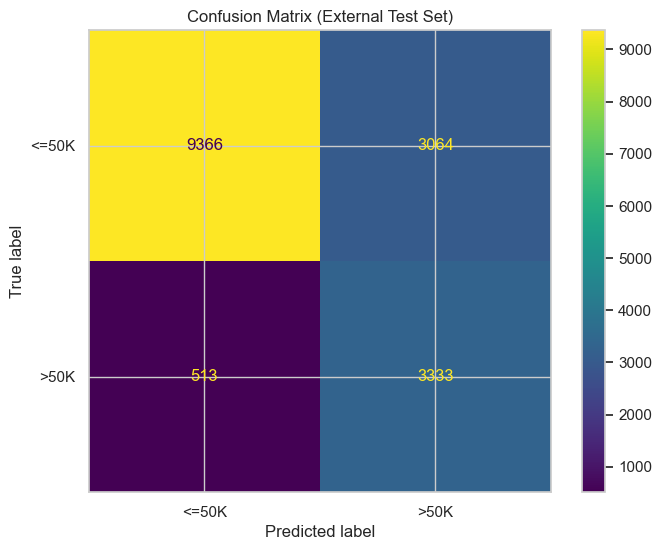
\includegraphics[width=0.8\textwidth]{images/svm_1.png}
\caption{Confusion matrix of the SVM model on the test data.}
\label{fig:svm_confusion_matrix}
\end{figure}

In summary, the SVM model demonstrated a strong capacity for classifying individuals based on income levels with satisfactory precision and recall. Future work may involve exploring kernel SVMs to handle non-linearly separable data and implementing cross-validation to refine hyperparameter selection.



\section{Results and Discussion}
This section presents a comprehensive summary of the findings from the logistic regression, Gaussian Naive Bayes, and Support Vector Machine models. Each model aimed to predict whether individuals earn more or less than \$50,000 per year based on U.S. Census data.

\subsection{Results Summary}
\begin{itemize}
    \item \textbf{Logistic Regression:} Achieved an accuracy of 79\% with the area under the ROC curve at 0.88. This model was particularly effective at distinguishing higher earners with robust precision and recall balance.
    \item \textbf{Gaussian Naive Bayes:} While traditionally faster and simpler, this model yielded slightly less accuracy overall compared to logistic regression but proved quick and effective for initial assessments.
    \item \textbf{Support Vector Machine:} Demonstrated the highest accuracy among the models at 80\%. It was particularly effective in handling the high-dimensional space of encoded categorical features, providing the best precision and recall metrics.
\end{itemize}

\subsection{Discussion}
The results indicate that while all models perform adequately, SVM stands out in terms of precision and accuracy, suggesting its suitability for datasets with a clear margin of separation among classes. Logistic regression, offering a good balance between computational efficiency and predictive power, is recommended for initial explorations and smaller datasets.

However, the Gaussian Naive Bayes model, despite its simplicity and speed, struggled with the skewed distribution of some features, indicating the need for data transformation or alternative methods that handle such distributions better.

The choice of model ultimately depends on the specific requirements of the task, including computational resources, the need for interpretability, and the expected data structure.

\section{Conclusion}
The analysis of the U.S. Census Income dataset through various statistical learning methods has provided valuable insights into the factors influencing income levels in the United States. While each model presented strengths and weaknesses, the combined use of these models can offer a more robust understanding of the underlying patterns.

\textbf{Limitations:}
\begin{itemize}
    \item The models could benefit from further tuning of hyperparameters and inclusion of interaction terms which might uncover more complex relationships.
    \item The dataset, being from 1994, might not fully represent the current economic conditions and demographics of the United States.
\end{itemize}

\textbf{Future Research:}
Future studies could focus on more recent datasets and consider the integration of additional socioeconomic variables, such as geographical data or newer indicators of economic activity. Further, employing advanced machine learning techniques like ensemble methods or deep learning could enhance the predictive performance and uncover deeper insights.

\section{References}
\begin{enumerate}
    \item U.S. Census Bureau. (1994). 1994 Census Database.
    \item EdPrice-MSFT. (n.d.). Introduction to Predictive Maintenance in Manufacturing - Azure Architecture Center. Microsoft Learn. Retrieved from \url{https://learn.microsoft.com/en-us/azure/architecture/industries/manufacturing/predictive-maintenance-overview}
    \item Bisong, E. (2019). Logistic regression. In \textit{Building Machine Learning and Deep Learning Models on Google Cloud Platform} (pp. 243-250). Apress, Berkeley, CA.
\end{enumerate}

\end{document}


